    
    \begin{frame}{Kódování}
    
    \begin{itemize}[<+->]
        \item Pro kódování TM $M=(Q,\{0,1\},\Gamma, \delta,q_1,B,\{q_2\})$ očíslujeme stavy, symboly a směry $L,R$.
    \item Předpokládejme:
    \begin{itemize}
        \item Počáteční stav je vždy $q_1$.
        \item Stav $q_2$ je vždy jediný koncový stav (nepotřebujeme víc, TM zastaví).
        \item První symbol je vždy 0, druhý 1, třetí B, prázdný symbol. Ostatní symboly pásky očíslujeme libovolně.
        \item Směr L je 1, směr R je 2.
    \end{itemize}
    \item Jeden krok $\delta(q_i,X_j)=(q_k,X_l,D_m)$ kódujeme: $0^i10^j10^k10^l10^m$. Všechna $i,j,k,l,m\geq 1$ takže se dvě jedničky za sebou nevyskytují.
    \item Celý TM se skládá z kódů všech přechodů v nějakém pořadí oddělených dvojicemi jedniček $11$: $C_111C_211\ldots C_{n-1}11C_n$.
    \end{itemize}\pause
    Budeme potřebovat uspořádat řetězce do posloupnosti:
    \begin{itemize}[<+->]
        \item Řetězce bereme uspořádané podle délky, stejně dlouhé uspořádáme lexikograficky.
    \item První je $\epsilon$, druhý $0$, třetí $1$, čtvrtý $00$ atd.
    \item $i$--tý řetězec označujeme $w_i$.
    \end{itemize}
    
    \end{frame}
    
    \begin{frame}{Příklad kódování TM}
    \begin{block}{Turingův stroj}
    $M=(\{q_1,q_2,q_3\},\{0,1\},\{0,1,B\},\delta,q_1,B,\{q_2\})$
    \begin{tabular}{r |c |c |c }
    $\delta$ & 0 & 1 & B \\
    \hline\hline
    $\rightarrow q_1$& & $(q_3,0,R)$& \\
    $*q_2$& & & \\
    $q_3$& $(q_1,1,R)$&$(q_2,0,R)$ &$(q_3,1,L)$.
    \end{tabular}
    \end{block}\pause
    \begin{itemize}
        \item 
    Kód pro transakce:
    \begin{tabular}{c |c |c |c }
    $C_1$&$C_2$&$C_3$&$C_4$\\
    0100100010100&
    0001010100100&
    00010010010100&
    0001000100010010
    \end{tabular}\pause
    \item 
    Kód celého TM:\\
    01001000101001100010101001001100010010010100110001000100010010.
    \end{itemize}
    \end{frame}
    
    \begin{frame}%{The Diagonal Language}
    \vskip-0.2cm
    \begin{definition}[Diagonální jazyk]
    \pojem{Diagonální jazyk $L_d$} je definovaný $L_d=\{w\in \{0,1\}^*; \hbox{TM reprezentovaný jako } w \hbox{ který nepřijímá slovo }w\}$.
    \end{definition}
    %\pause
    \begin{minipage}{0.35\textwidth}
    $L_d=\{w; \hbox{na diagonále je } 0\}$.
    \begin{theorem}
    $L_d$ není rekurzivně spočetný jazyk, tj. neexistuje TM přijímající $L_d$.
    \end{theorem}
    $i$ - k\'od TM\\
    $j$ - vstup $w$\\
    0/1 - prijima/neprijema\\
    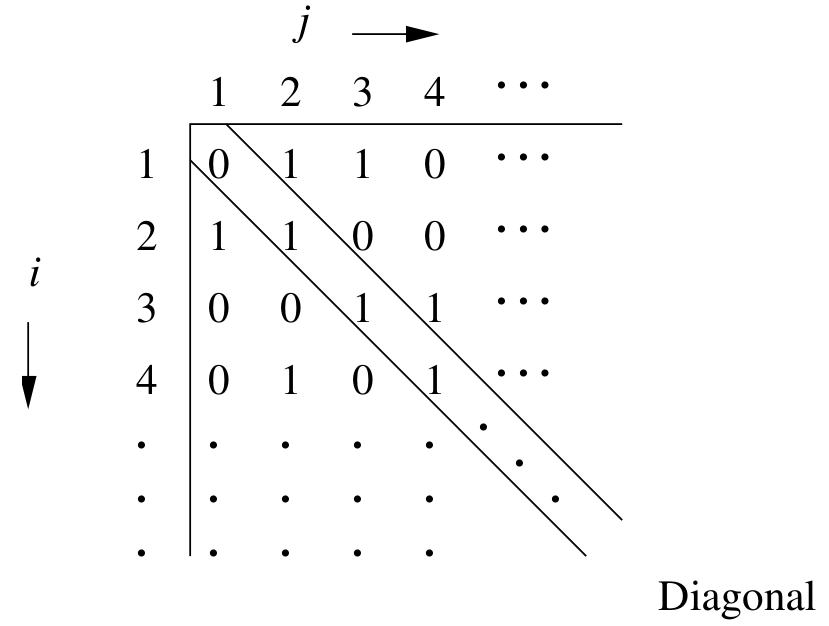
\includegraphics[width=\textwidth]{diagonal.PNG}
    \end{minipage}
    \begin{minipage}{0.03\textwidth}
    \ \end{minipage}
    \begin{minipage}{0.6\textwidth}
    \begin{proof}
    \begin{itemize}%[<+->]
        \item Předpokládejme $L_d$ je RE, $L_d=L(M_d)$ pro nějaký TM $M_d$.
        \item Jeho jazyk je $\{0,1\}$, tedy je v seznamu na obrázku: 'Přijímá TM $M_i$ vstupní slovo $w_j$?'
        \item Alespoň jeden řetězec ho kóduje, řekněme $code(M_d)=w_d$.
        \item Je $w_d\in L_d$
        
        \begin{itemize}
            \item Pokud 'ano', na diagonále má být 0, tj. $w_d\notin L(M_d)=L_d$, spor.
    \item Pokud 'ne', na diagonále má být 1, $w_d\in L(M_d)=L_d$, spor.
        \end{itemize}
     %\pause
        Proto takový $M_d$ neexistuje. Tedy $L_d$ není rekurzivně spočetný.
    \end{itemize}
    \end{proof}
    \end{minipage}
    \end{frame}
    %An Undecidable Problem That Is RE
    %\begin{frame}{Základní hierarchie jazyků}
    %\begin{minipage}{0.6\textwidth}
    %Základní typy jazyků:
    %\begin{itemize}
        %\item Rekurzivní, rozhodnutelný: Přijímaný TM který vždy zastaví, ať už vstup přijme nebo nepřijme.
        %\item RE Rekurzivně spočetný: přijímaný nějakým TM. Výpočet může trvat, nikdy nevíme, jestli je slovo zamítnuto nebo máme ještě čekat.
        %\item Některé jazyky nejsou ani rekurzivně spočetné, {\em non}-RE jazyky, jako $L_d$ is {\em non}--RE jazyk.
    %\end{itemize}
    %\end{minipage}
    %\begin{minipage}{0.03\textwidth}
    %\ \end{minipage}
    %\begin{minipage}{0.3\textwidth}
    %\includegraphics[width=\textwidth]{languages.PNG}
    %\end{minipage}
    %\end{frame}
    
    
    
    \begin{frame}{Univerzální Turingův stroj}
    \begin{definition}[Univerzální jazyk]
    Definujeme \pojem{univerzální jazyk} $L_u$ jakožto množinu binárních řetězců které kódují pár $(M,w)$, kde $M$ je TM a $w \in L(M)$.
    
    TM přijímající $L_u$ se nazývá \pojem{Univerzální Turingův stroj}.
    \end{definition}
    \pause
    \begin{theorem}[Existence Univerzálního Turingova stroje]
    Existuje Turingův stroj $U$, pro který $L_u=L(U)$.
    \end{theorem}
    \begin{minipage}{0.37\textwidth}
    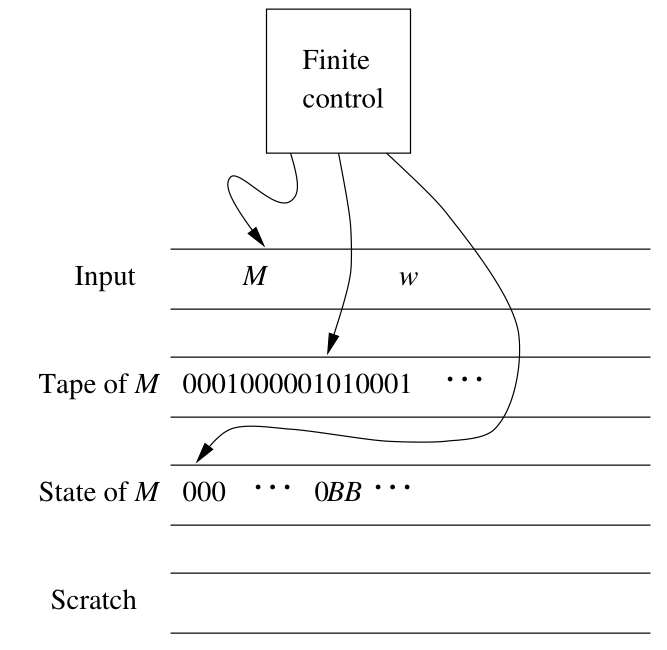
\includegraphics[width=\textwidth]{universalTM.PNG}
    \end{minipage}
    \begin{minipage}{0.01\textwidth}
    \end{minipage}
    \begin{minipage}{0.61\textwidth}
    Popíšeme $U$ jako vícepáskový Turingův stroj.
    \begin{itemize}[<+->]
        \item Přechody $M$ jsou napsány na první pásce spolu s řetězcem $w$.
        \item Na druhé pásce simulujeme výpočet $M$, používající formát jako kód $M$, tj. symboly $0^i$ oddělené jedničkou $1$.
        \item Třetí páska obsahuje stav $M$ reprezentovaný $i$ nulami.
    \end{itemize}
    \end{minipage}
    \end{frame}
    
    \begin{frame}{Operace univerzálního Turingova stroje}
    %\begin{minipage}{0.79\textwidth}
    Operace $U$ jsou následující:
    \begin{itemize}[<+->]
        \item Otestuj, zda je kód $M$ legitimní;\\ pokud ne, $U$ zastav bez přijetí.
        \item Inicializuj druhou pásku kódovaným slovem $w$: $10$ pro $0$ ve $w$, $100$ pro $1$; blank jsou nechané prázdné a nahrazeny $1000$ pouze 'v případě potřeby'.
        \item Napiš $0$, počáteční stav $M$, na třetí pásku. Posuň hlavu druhé pásky na první simulované políčko.
        \item Simuluj jednotlivé přechody $M$
        \begin{itemize}
            \item Najdi na první pásce správnou transakci $0^i10^j10^k10^l10^m$, $0^i$ na pásce 3, $0^j$ na pásce 2.
            \item Změň obsah pásky 3 na $0^k$.
            \item Nahraď $0^j$ na 2. pásce řetězcem $0^l$. Použij čtvrtou 'scratch tape' pro správné mezery.
            \item Posuň hlavu 2. pásky na pozici vedle $1$ vlevo nebo vpravo, podle pohybu $m$.
        \end{itemize}
            \item Pokud jsme nenašli instrukci pro $M$, zastavíme.
            \item Pokud $M$ přejde do přijímajícího stavu, pak  $U$ také přijme.\qed
    \end{itemize}
    %\end{minipage}
    \begin{tikzpicture}[overlay]
    \node at (10,7.3) {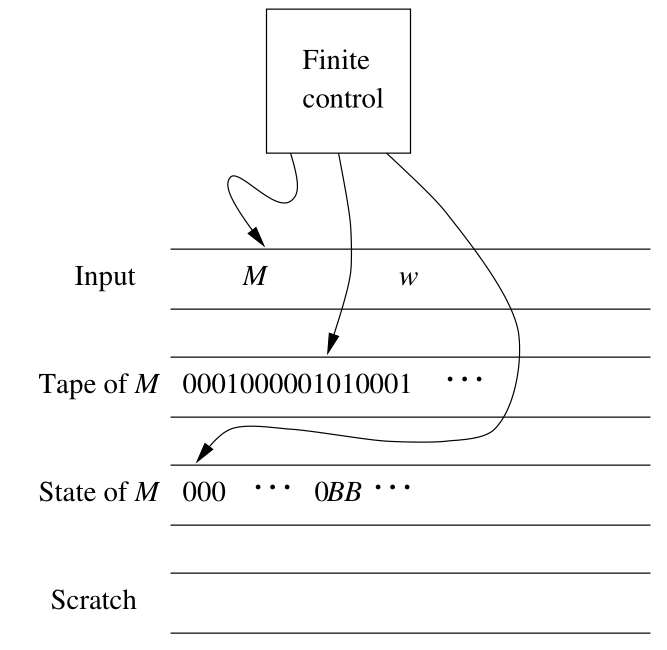
\includegraphics[width=2.5cm]{universalTM.PNG}};
    \end{tikzpicture}
    \end{frame}
    
    \begin{frame}{$L \& \overline{L}\in RE \Rightarrow L, \overline{L}$ je rekurzivní}
    \begin{minipage}{0.55\textwidth}
    \begin{lemma}
    Je--li $L$ rekurzivní jazyk, je rekurzivní i $\bar{L}$.
    \end{lemma}
    \end{minipage}\pause
    \begin{minipage}{0.03\textwidth}
    \ \end{minipage}
    \begin{minipage}{0.4\textwidth}
    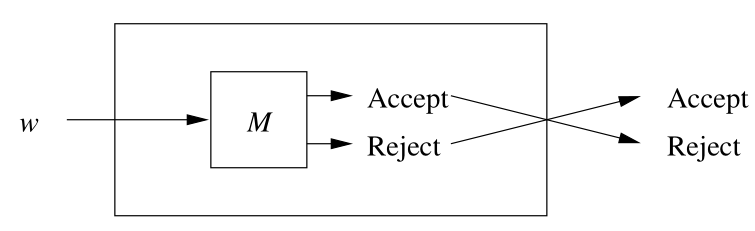
\includegraphics[width=\textwidth]{compRec.PNG}
    \end{minipage}
    \begin{minipage}{0.55\textwidth}
    \begin{theorem}[Postova věta]
    Jazyk $L$ je rekurzivní, právě když $L$ i $\overline{L}$ (doplněk) jsou rekurzivně spočetné.
    \end{theorem}
    \end{minipage}\hfill\pause
    \begin{minipage}{0.3\textwidth}
    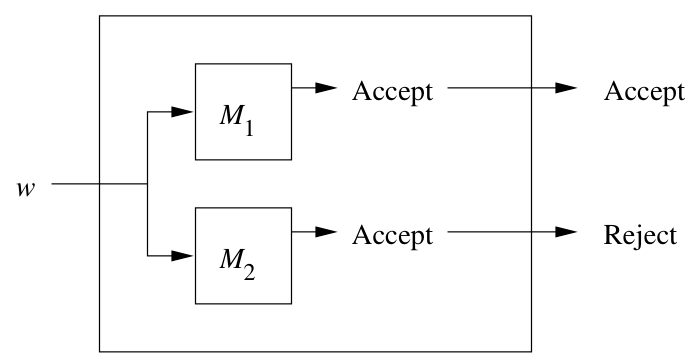
\includegraphics[width=\textwidth]{bothRE.PNG}
    \end{minipage}
    \begin{proofm}{}
    \begin{itemize}[<+->]
        \item Máme TM $L=L(M_1)$ a $\overline{L}=L(M_2)$.
        \item pro dané slovo $w$ naráz simulujeme $M_1$ i $M_2$ (dvě pásky, stav se dvěma komponentami).
        \item Pokud jeden z $M_i$ přijme, $M$ zastaví a odpoví.
        \item Jazyky jsou komplementární, jeden z $M_i$ vždy zastaví, $L$ je rekurzivní.
    \end{itemize}
    \end{proofm}
    \end{frame}
    
    
    
    \begin{frame}{Nerozhodnutelnost univerzálního jazyka}
    \begin{theorem}[Nerozhodnutelnost univerzálního jazyka]
    $L_u$ je rekurzivně spočetný, ale není rekurzivní.
    \end{theorem}
    \begin{minipage}{0.5\textwidth}
    \begin{proof}
    \begin{itemize}[<+->]
        \item Máme TM přijímající $L_u$, tj. je RE.
            \item Předpokládejme, že je $L_u$ rekurzivní.
            \item Pak $\overline{L_u}$ by byl také rekurzivní.
            \item Pro TM přijímající $\overline{L_u}$ můžeme zkonstruovat TM přijímající $L_d$ (vpravo). 
            \item Protože víme, že $L_d$ není RE, $\overline{L_u}$ není RE a $L_u$ není rekurzivní.
    \end{itemize}
    \end{proof}
    \end{minipage}
    \pause
    \begin{minipage}{0.01\textwidth}
    \end{minipage}
    \begin{minipage}{0.48\textwidth}
    Modifikace TM pro $\overline{L_u}$ na TM pro $L_d$:
    \includegraphics[width=\textwidth]{LU.PNG}
    \begin{itemize}[<+->]
        \item Řetězec $w$ přepiš na $w111w$ (2--páskový, převeď na 1--páskový).
        \item Simuluj M na novém vstupu. Přijmi iff $M$ přijme.
        \item %Zvol $i$ tak že $w_i=w$. 
    Stroj $M'$ přijímá $\overline{L_u}(w,w)$, tj. případy kdy  $M_i$ nepřijímá $w_i$, tj. jazyk $L_d$.
    \end{itemize}
    \end{minipage}
    \end{frame}




    
\begin{frame}{Nerozhodnutelné problémy o automatech a gramatikách}
    \begin{definition}[Rozhodnutelný problém]
    \pojem{Problémem} $P$ myslíme matematicky/informaticky definovanou množinu otázek kódovatelnou řetězci nad abecedou $\Sigma$ s odpověďmi $\in\{ano, ne\}$.
    %\pause
    
    \pojem{Problém je (algoritmicky) rozhodnutelný}, pokud existuje Turingův stroj TM takový, že pro každý vstup $w\in P$ zastaví a navíc přijme právě když $P(w)=ano$ (tj. pro $P(w)=ne$ zastaví v ne--přijímacím stavu).
    
    Problém který není algoritmicky rozhodnutelný nazýváme \pojem{nerozhodnutelný problém}.
    \end{definition}
    %\pause
    'Rozhodnutelný' mluví o problémech, 'rekurzivní' o jazycích, jinak jde o 'totéž'.
    \begin{example}['Problémy']
    \begin{itemize}%[<+->]
        \item Obsahuje vstupní slovo pět nul?
        \item Je vstupní slovo korektně definovaným kódem Turingova stroje v kódování výše?
        \item Zastaví TM kódu $M$ nad slovem $w$?
        \item Zastaví TM kódu $w$ nad slovem $w$?
    \end{itemize}
    \end{example}
    \end{frame}
    
    \begin{frame}{Redukce}
    \begin{minipage}{0.57\textwidth}
    \begin{definition}[Redukce]
    \pojem{Redukcí problému} $P_1$ na $P_2$, nazýváme algoritmus $R$, který pro každou instanci $w\in P_1$ zastaví a vydá $R(w)\in P_2$
    tak, že 
    \begin{itemize}
        \item $P_1(w)=ano$ právě když $P_2(R(w))=ano$ 
        \item tj. i $P_1(w)=ne$ právě když $P_2(R(w))=ne$. 
    \end{itemize}
    \end{definition}
    %\pause
    \end{minipage}
    \begin{minipage}{0.01\textwidth}
    \end{minipage}
    \begin{minipage}{0.41\textwidth}
    \includegraphics[width=\textwidth]{reduction.PNG}
    \end{minipage}
    \begin{example}
    \begin{minipage}{0.48\textwidth}
    Redukce  TM pro $L_d$ na  TM pro $\overline{L_u}$:
    \includegraphics[width=\textwidth]{LU.PNG}
    \end{minipage}
    \begin{minipage}{0.01\textwidth}
    \end{minipage}
    \begin{minipage}{0.41\textwidth}
    \begin{itemize}
        \item $P_1=$ Nepřijímá TM reprezentovaný $w$ vstupní slovo $w$?
        \item $P_2=$ Nepřijímá TM reprezentovaný $M$ vstupní slovo $w$?
        \end{itemize}
    \end{minipage}
    \end{example}
    \end{frame}
    
    \begin{frame}{Věta o (ne)rozhodnutelnosti díky redukci}
    \begin{minipage}{0.57\textwidth}
    \begin{theorem}[Redukce]
    Pokud existuje redukce problému $P_1$ na $P_2$, pak:
    \begin{itemize}%[<+->]
        \item Pokud $P_1$ je nerozhodnutelný, pak je nerozhodnutelný i $P_2$. 
        \item Pokud $P_1$ není rekurzivně spočetný, pak není RE ani $P_2$. 
    \end{itemize}
    \end{theorem}
    \end{minipage}
    \begin{minipage}{0.01\textwidth}
    \end{minipage}
    \begin{minipage}{0.41\textwidth}
    \includegraphics[width=\textwidth]{reduction.PNG}
    \end{minipage}
    \begin{proof}
    \begin{itemize}%[<+->]
        \item Předpokládejme $P_1$ je nerozhodnutelný. Je--li možné rozhodnout $P_2$, pak můžeme zkombinovat redukci  $P_1$ na $P_2$ s algoritmem rozhodujícím $P_2$ pro konstrukci algoritmu rozhodujícího $P_1$. Proto je $P_2$ nerozhodnutelný.
        \item Předpokládejme $P_1$ ne--RE, ale $P_2$ je RE. Podobně jako výše zkombinujeme redukci a výsledek $P_2$  k důkazu $P_1$ je RE; SPOR.
    \end{itemize}
    \end{proof}
    \end{frame}
    
    \begin{frame}{Problém zastavení}
    %\begin{theorem*}[Nerozhodnutelnost univerzálního jazyka]
    %%%%%%%%Víme: $L_u$ je rekurzivně spočetný, ale není rekurzivní.
    %\pause
    %\end{theorem*}
    \begin{definition}[Problém zastavení]
    \pojem{Instancí problému zastavení} je dvojice řetězců $M,w\in \{0,1\}^*$.\\ \pojem{Problém zastavení} je najít alogritmus $Halt(M,w)$, který vydá $1$ právě když stroj $M$ zastaví na vstupu $w$, jinak vydá $0$.
    \end{definition}
    %\pause
    \begin{theorem*}[Problém zastavení]
    Problém zastavení není rozhodnutelný.
    \end{theorem*}
    %\pause
    
    
    \begin{proof}
    \begin{itemize}%[<+->]
        \item Redukujeme $L_d$ na $Halt$.
            \item Předpokládejme, že máme algoritmus (Turingův stroj) pro $Halt()$.
            \item Modifikujeme ho na stroj $Halt_{no}(w)$; $w\in \{0,1\}^*$:
        \begin{itemize}
            \item Pokud $Halt(w,w)$, spustíme nekonečný cyklus
            \item jinak zastavíme.
        \end{itemize}
        \item Otázka $Halt(Halt_{no}, Halt_{no})$ není řešitelná, proto algoritmus $Halt()$ nemůže existovat.
    \end{itemize}
    \end{proof}
    \end{frame}
    
    %
    %\begin{frame}{TM přijímající prázdný jazyk (nic)}
    %\begin{definition}
    %Slova $w$ jazyků $L_e, L_{ne}\in \{0,1\}^*$  vnímáme jako kódy Turingových strojů. Definujeme:
    %\begin{itemize}
        %\item $L_e=\{w|L(w)=\emptyset\} $
        %\item $L_{ne}=\{w|L(w)\neq\emptyset\} $.
    %\end{itemize}
    %\end{definition}
    %%\pause
    %
    %\begin{minipage}{0.45\textwidth}
    %\begin{theorem}
    %$L_{ne}$ je rekurzivně spočetný (RE).
    %\end{theorem}
    %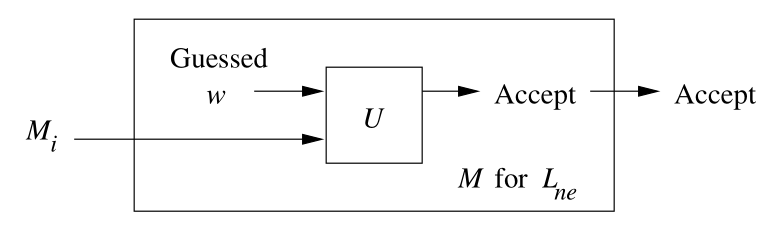
\includegraphics[width=\textwidth]{Lne.PNG}
    %\begin{theorem}%<3->
    %$L_{e}$ není rekurzivně spočetný, proto $L_{ne}$ není rekurzivní.
    %\end{theorem}
    %\end{minipage}
    %\begin{minipage}{0.01\textwidth}
    %\ \end{minipage}
    %\begin{minipage}{0.51\textwidth}
    %%\pause 
    %Redukce: Pro $w\in L_d$ do $M; L(M)=L_{e}$.
    %\pause
    %\begin{itemize}
        %\item Obraz $R(w)$ je TM, který ignoruje svůj vstup $x$,
    %%\pause
        %\item na vstupní pásku napíše $w$ a simuluje $U$ na vstupu $w$.
    %%\pause
        %\item Jazyk je prázdný iff stroj $w$ nepřijímá $w$, tj. přijímá diagonální jazyk.
    %\end{itemize}
    %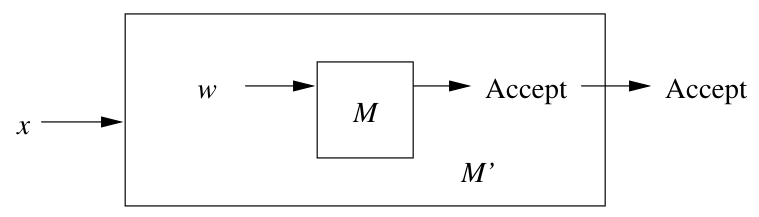
\includegraphics[width=\textwidth]{Lne2.PNG}
    %\end{minipage}
    %\end{frame}
    
    %
    %\begin{frame}{Properties of the RE Languages}
    %\begin{definition}{Properties of the RE Languages}
    %A \pojem{property} of the RE languages is simply a set of RE languages.
    %
    %A property is \pojem{trivial} if it is either empty, or is all RE languages. Otherwise, it is \pojem{nontrivial}.
    %\end{definition}
    %\begin{example}[Examples:]
    %\begin{itemize}
        %\item Being context--free language CFL.
        %\item The property of being empty is the set $\{\emptyset\}$. 
        %\item Empty property $\emptyset$.
    %\end{itemize}
    %\end{example}  
    %\begin{theorem}[Rice's Theorem]
    %Every nontrivial property of the RE languages is undecidable.
    %\end{theorem}
    %\end{frame}
    %
    %
    %\begin{frame}{Rice's Theorem}
    %\begin{minipage}{0.48\textwidth}
    %\begin{theorem}[Rice's Theorem]
    %Every nontrivial property of the RE languages is undecidable.
    %\end{theorem}
    %\end{minipage}
    %\begin{minipage}{0.01\textwidth}
    %\end{minipage}
    %\begin{minipage}{0.48\textwidth}
    %\includegraphics[width=\textwidth]{rice.PNG}
    %\end{minipage}
    %\begin{proof}
    %\begin{itemize}
        %\item Let ${\cal P}$ be a nontrivial property of the RE languages, assume $\emptyset \notin {\cal P}$, $L \in {\cal P}$, $M_L$ a TM accepting $L$.
        %\item We construct $M'$, two tape TM on the figure, reducing $L_u$ to $L_{\cal P}$.
        %
        %\begin{itemize}
            %\item First tape is used to simulate $M$ on $w$.
            %\item If $M$ does not accept $w$, $M'$ does nothing else, so $L(M')=\emptyset$ and from assumption $\emptyset \notin{\cal P}$, that means the code for M' is not in $L_{\cal P}$.
                %\item If $M$ accepts $w$, then $M'$ begins simulating $M_L$ on its own input $x$. Thus, $M'$ will accept exactly the language $L$. Since $L\in {\cal P}$, the code for M' is in $L_{\cal P}$. 
        %\end{itemize}
        %\item If $\emptyset \in {\cal P}$, then $\emptyset \notin \overline{\cal P}$. From above, $\overline{\cal P}$ is undecidable, it is RE. Then, the complement $L_{\cal P}$ must be undecidable.
    %\end{itemize}
    %\end{proof}
    %\end{frame}
    
    
    
    \begin{frame}{Směřujeme k nerozhodnutelným problémům o bezkontextových gramatikách}
    
    \includegraphics[width=4cm]{PCP.PNG}
    \begin{itemize}
        \item Ne-rozhodnutelnost univerzálního jazyka
     \item redukujeme na modifikovaný PCP (MPCP)
     \item což redukujeme na PCP
     \item což redukujeme na otázku $L(G_1)\cap L(G_2)$ pro dvě bezkontextové gramatiky
     \begin{itemize}\item a další podobné otázky.
    \end{itemize}
    \end{itemize}
    \end{frame}
    
    
    
    \begin{frame}{Postův korespondenční problém}
    \begin{definition}[Postův korespondenční problém]
    Instance \pojem{Postova korespondenčního problému (PCP)} jsou dva seznamy slov nad abecedou $\Sigma$ značené $A=w_1,w_2,\ldots, w_k$ a $B=x_1,x_2,\ldots, x_k$ stejné délky $k$. 
    \pause
    Pro každé $i$, dvojice $(w_i,x_i) $ se nazývá \pojem{odpovídající} dvojice. 
    \pause
    
    Instance PCP \pojem{má řešení}, pokud existuje posloupnost jednoho či více přirozených čísel ${i_1}, {i_2}, \ldots, {i_m}$ tak že $w_{i_1} w_{i_2} \ldots w_{i_m}=x_{i_1} x_{i_2} \ldots x_{i_m} $ tj. dostaneme stejné slovo.
    \pause
    V tom případě říkáme, že posloupnost ${i_1}, {i_2}, \ldots, {i_m}$  \pojem{je řešení}.
    \pause
    
    \pojem{Postův korespondenční problém} je: Pro danou instanci PCP, rozhodněte, zda má řešení.
    \end{definition}
    \pause
    \begin{example}
    \begin{minipage}{0.37\textwidth}
    \begin{tabular}{c | l | l}
     & Seznam $A$ & Seznam $B$\\
    \hline
    $i$ & $w_i$ & $x_i$ \\
    \hline
    1 & 1 & 111\\
    2 & 10111 & 10\\
    3 & 10 & 0 
    \end{tabular}
    \end{minipage}
    \begin{minipage}{0.01\textwidth}
    \ \end{minipage}
    \begin{minipage}{0.51\textwidth}
    \begin{itemize}
        \item $\Sigma=\{0,1\}$, seznamy A,B v tabulce.
        \item Řešení $2,1,1,3$ vytvoří slovo 101111110.
        \item Jiné řešení: 2,1,1,3,2,1,1,3.
    \end{itemize}
    \end{minipage}
    \end{example}
    \end{frame}
    
    \begin{frame}{Částečná řešení}
    \vskip-0.5cm
    \begin{minipage}{0.3\textwidth}
    \begin{example}
    $\Sigma=\{0,1\}$. Neexistuje řešení pro seznamy:
    \begin{tabular}{c | l | l}
     & List $A$ & List $B$\\
    \hline
    $i$ & $w_i$ & $x_i$ \\
    \hline
    1 & 10 & 101\\
    2 & 011 & 11\\
    3 & 101 & 011. 
    \end{tabular}
    \end{example}
    \pause
    Zdůvodnění:
    \begin{itemize}
        \item $i_{1}=1$, jinak by první symbol neodpovídal.
    \pause
        \item Máme částečné řešení:
    \begin{tabular}{ l}
    A: $10\cdots$\\
    B: $101\cdots$
    \end{tabular}
    \end{itemize}
    \end{minipage}
    \pause
    \begin{minipage}{0.01\textwidth}
    \ \end{minipage}
    \begin{minipage}{0.67\textwidth}
    \begin{definition}[Částečné řešení]
    \pojem{Částečným řešením} nazýváme posloupnost indexů ${i_1}, {i_2}, \ldots, {i_r}$ taková že jeden z řetězců $w_{i_1}, w_{i_2}, \ldots, w_{i_r}$ a $x_{i_1}, x_{i_2},\ldots, x_{i_r} $ je prefix druhého (i v případě, že řetězce nejsou totožné).
    \end{definition}
    \pause
    \begin{lemma}
    Je--li posloupnost čísel řešením, pak je každý prefix částečným řešením.
    \end{lemma}
    \pause
    \begin{minipage}{0.59\textwidth}
    \begin{itemize}[<+->]
        \item $i_{2}=1$, řetězce \begin{tabular}{l}1010\\101101\end{tabular} nesouhlasí na 4.pozici.
        \item $i_{2}=2$, \begin{tabular}{l}10011\\10111\end{tabular} nesouhlasí na 3.pozici.
    \item Je možné jen $i_2=3$.
    \end{itemize}
     \end{minipage}
    \begin{minipage}{0.4\textwidth}
    \begin{tabular}{ l}
    A: $10101\cdots$\\
    B: $101011\cdots$
    \end{tabular}
    \begin{itemize}[<+->]
        \item Jsme ve stejné pozici jako po volbě $i_1=1$. 
        \item Nelze dostat oba řetězce na stejnou délku.
    \end{itemize}
     \end{minipage}
     \end{minipage}
    
    \end{frame}
    
    \begin{frame}{Modifikovaný Postův korespondenční probém MPCP}
    \begin{definition}[Modifikovaný Postův korespondenční probém MPCP]
    Mějme PCP, tj. seznamy $A=w_1,w_2,\ldots, w_k$ a $B=x_1,x_2,\ldots, x_k$. Hledáme seznam 0 nebo více přirozených čísel  ${i_1}, {i_2}, \ldots, {i_m}$ tak že ${\bf w_1,}w_{i_1}, w_{i_2}, \ldots, w_{i_m}={\bf x_1,}x_{i_1}, x_{i_2}, \ldots, x_{i_m} $. V tom případě říkáme, že PCP \pojem{má iniciální řešení}.
    
    \pojem{Modifikovaný Postův korespondenční problém}: má PCP iniciální řešení?
    \end{definition}
    \begin{minipage}{0.37\textwidth}
    \begin{example}
    Tento PCP nemá iniciální řešení.\\
    \begin{tabular}{c | l | l}
     & seznam $A$ & seznam $B$\\
    \hline
    $i$ & $w_i$ & $x_i$ \\
    \hline
    1 & 1 & 111\\
    2 & 10111 & 10\\
    3 & 10 & 0 
    \end{tabular}
    \end{example}
    \end{minipage}\hfill
    \begin{minipage}{0.57\textwidth}
    \begin{proofm}{}
    \begin{itemize}
        \item  Částečné instance 
    \begin{tabular}{l}1\\111\end{tabular}, 
    \begin{tabular}{l}11\\111111\end{tabular} se nikdy nesrovnají na stejnou délku. 
    \item Jiné volby vedou k různým písmenům abecedy.
    \end{itemize}
    \end{proofm}
    \end{minipage}
    \end{frame}
    
    \begin{frame}{MPCP redukce na PCP}
    \vspace{-0.5cm}
    \begin{minipage}{0.45\textwidth}
    \begin{lemmaN}[Red. MPCP na PCP]\label{lemMPCA}
    $w\in MPCP$ má iniciální řešení, právě když má $R(w)$ řešení.
    \end{lemmaN}
    %The same lists as before as a MPCP.\\
    \begin{tabular}{c | l | l}
     & List $A$ & List $B$\\
    \hline
    $i$ & $w_i$ & $x_i$ \\
    \hline
    1 & 1 & 111\\
    2 & 10111 & 10\\
    3 & 10 & 0 
    \end{tabular}
    \end{minipage}
    \begin{minipage}{0.01\textwidth}
    \ \end{minipage}
    \pause
    \begin{minipage}{0.52\textwidth}
    \begin{example}[MPCP redukce na PCP.]
    \begin{tabular}{c | l | l}
     & List $C$ & List $D$\\
    \hline
    $i$ & $y_i$ & $z_i$ \\
    \hline
    0 & *1* & *1*1*1\\
    1 & 1* & *1*1*1\\
    2 & 1*0*1*1*1* & *1*0\\
    3 & 1*0* & *0\\
    4 & \$ & *\$ 
    \end{tabular}
    \end{example}
    \end{minipage}
    \begin{proofm}{}
    \begin{itemize}[<+->]
        \item Vezměme nové symboly $*,\$\notin \Sigma$.
        \item  $\forall i=1,\ldots,k$ definujeme $y_i$ rozšířením $w_i$ s $*$ za každým písmenem $w_i$.
        \item  $\forall i=1,\ldots,k$ def. $z_i$ rozšířením $x_i$ s $*$ \textbf{před} každým písmenem $x_i$.
        \item $y_0=*y_1$, $z_0=z_1$.
        \item $y_{k+1}=\$$, $z_{k+1}=*\$$.
        \item ${i_1}, {i_2}, \ldots, {i_m}$ je iniciální řešení, iff $0,{i_1}, {i_2}, \ldots, {i_m},(k+1)$ je řešení PCP.
    \end{itemize}
    \end{proofm}
    \end{frame}
    
    \begin{frame}{Nerozhodnutelnost PCP }
    \vspace{-0.2cm}
    \begin{itemize}[<+->]
        \item Chceme dokázat, že PCP je algoritmicky nerozhodnutelný.
        \item Redukovali jsme MPCP na PCP (minulý slajd)
        \item a redukujeme $L_u$ na MPCP.
    %	\item Since $L_u$ is undecidable, the PCP must be undecidable too.
    \end{itemize}
    \vspace{-2mm}
    \begin{algm}{Redukce $L_u$ na MPCP}
    Konstruujeme MPCP pro TM  $M=(Q,\Sigma,\Gamma, \delta,q_0,B,F)$, který nikdy nepíše $B$ a nejde hlavou doleva od počáteční pozice.
    Nechť $w\in \Sigma^*$ je vstupní slovo.
    \pause
    \begin{tabular}{ l  l l}
     seznam $A$ & seznam $B$\\
    \# & \#$q_0w$\#\\
    \hline
    $X$ & $X$ & $\forall$ $X\in \Gamma$\\
    \# & \#\\
    \hline
    $qX$ & $Yp$ & pro $\delta(q,X)=(p,Y,R) $\\
    $ZqX$ & $pZY$ & pro $\delta(q,X)=(p,Y,L), Z \in \Gamma $ symbol pásky\\
    $q\#$ & $Yp\#$ & pro $\delta(q,B)=(p,Y,R) $\\
    $Zq\#$ & $pZY\#$ & pro $\delta(q,B)=(p,Y,L), Z \in \Gamma $ symbol pásky\\
    \hline
    $XqY$ & $q$& $q\in F$, přijímající stav\\
    $Xq$ & $q$& $q\in F$\\
    $qY$ & $q$& $q\in F$\\
    $q\#\#$ & $q\#$& $q\in F$.
    \end{tabular}
    \end{algm}
    \begin{tikzpicture}[overlay]
    \node at (10,7.3) {\includegraphics[width=4cm]{PCP.PNG}};
    \end{tikzpicture}
    %\includegraphics[width=\textwidth]{PCP.PNG}
    \end{frame}
    
    
    \begin{frame}{}
    \begin{minipage}{0.65\textwidth}
    \begin{example}Konvertujme TM $M=(\{q_1,q_2,q_3\},\{0,1\},\{0,1,X,Y,B\},\delta,q_1,B,\{q_3\})$
    \begin{tabular}{c | c |c| c }
    $q_i$ & $\delta(q_i,0)$ & $\delta(q_i,1)$ & $\delta(q_i,B)$ \\
    \hline 
    $q_1$ & $(q_2,1,R)$& $(q_2,0,L)$&  $(q_2,1,L)$\\
    $q_2$ & $(q_3,0,L)$ & $(q_1,0,R)$& $(q_2,0,R)$\\
    $q_3$ & -- & -- & -- 
    \end{tabular} 
    
    a vstupní slovo $w=01$ na instanci MPCP.
    \end{example}
    \pause
    \begin{tabular}{c  c |c| c }
     & seznam $A$ & seznam $B$ & zdroj\\
    \hline
     & $q_10$ & $1q_2$ & z $\delta(q_1,0)=(q_2,1,R)$ \\
     & $0q_11$ & $q_200$ & z $\delta(q_1,1)=(q_2,0,L)$ \\
     & $1q_11$ & $q_210$ & z $\delta(q_1,1)=(q_2,0,L)$ \\
     & $0q_1\#$ & $q_201\#$ & z $\delta(q_1,B)=(q_2,1,L)$ \\
     & $1q_1\#$ & $q_211\#$ & z $\delta(q_1,B)=(q_2,1,L)$ \\
     & $0q_20$ & $q_300$ & z $\delta(q_2,0)=(q_3,0,L)$ \\
     & $1q_20$ & $q_310$ & z $\delta(q_2,0)=(q_3,0,L)$ \\
     & $q_21$ & $0q_1$ & z $\delta(q_2,1)=(q_1,0,R)$ \\
     & $q_2\#$ & $0q_2\#$ & z $\delta(q_2,B)=(q_2,0,R)$ \\
    \hline
    \end{tabular} 
    \end{minipage}\hfill
    \pause
    \begin{minipage}{0.32\textwidth}
    Seznam dvojic bez $B$ symbolu (ve dvou tabulkách)\\
    \begin{tabular}{c c |c c}
     & seznam $A$ & seznam $B$ & \\
    \hline
    & \# & \#$q_101$\#\\
    & 0 & 0 &\\
    & 1 & 1 &\\
    & \# & \# &\\
    \hline
     & $0q_30$ & $q_3$ & \\
     & $0q_31$ & $q_3$ & \\
     & $1q_30$ & $q_3$ & \\
     & $1q_31$ & $q_3$ & \\
     & $0q_3$ & $q_3$ & \\
     & $1q_3$ & $q_3$ & \\
     & $q_30$ & $q_3$ & \\
     & $q_31$ & $q_3$ & \\
    \hline
     & $q_3\#\#$ & $\#$ & 
    \end{tabular} 
    \end{minipage}
    \end{frame}
    
    
    \begin{frame}{MPCP simulace TM}
    \begin{minipage}{0.65\textwidth}
    \begin{tabular}{c  c |c| c }
     & seznam $A$ & seznam $B$ & zdroj\\
    \hline
     & {\cellcolor{blue} $q_10$} & \cellcolor{blue}$1q_2$ & z $\delta(q_1,0)=(q_2,1,R)$ \\
     & $0q_11$ & $q_200$ & z $\delta(q_1,1)=(q_2,0,L)$ \\
     & $1q_11$ & $q_210$ & z $\delta(q_1,1)=(q_2,0,L)$ \\
     & {\cellcolor{violet}$0q_1\#$} & \cellcolor{violet}$q_201\#$ & z $\delta(q_1,B)=(q_2,1,L)$ \\
     & $1q_1\#$ & $q_211\#$ & z $\delta(q_1,B)=(q_2,1,L)$ \\
     & $0q_20$ & $q_300$ & z $\delta(q_2,0)=(q_3,0,L)$ \\
     & {\cellcolor{orange} $1q_20$} & \cellcolor{orange}$q_310$ & z $\delta(q_2,0)=(q_3,0,L)$ \\
     & {\cellcolor{red}$q_21$} & \cellcolor{red}$0q_1$ & z $\delta(q_2,1)=(q_1,0,R)$ \\
     & $q_2\#$ & $0q_2\#$ & z $\delta(q_2,B)=(q_2,0,R)$ \\
    \hline
    \end{tabular}
    
    \begin{itemize}
        \item $M$ přijímá posloupností $q_101\vdash 1q_21 \vdash 10q_1 \vdash 1q_201 \vdash q_3101$.
    \end{itemize}
    
    \end{minipage}
    \begin{minipage}{0.001\textwidth}
    \ \end{minipage}
    \begin{minipage}{0.32\textwidth}
    \begin{tabular}{c c |c c}
     & seznam $A$ & seznam $B$ & \\
    \hline
    & \# & \#$q_101$\#\\
    &\uncover<3->{\cellcolor{green}}0 & \cellcolor{green}0 &\\
    & \cellcolor{green}1 & \cellcolor{green}1 &\\
    & \cellcolor{green}\# & \cellcolor{green}\# &\\
    \hline
     & \cellcolor{cyan}$0q_30$ & \cellcolor{cyan}$q_3$ & \\
     & \cellcolor{cyan}$0q_31$ & \cellcolor{cyan}$q_3$ & \\
     & \cellcolor{cyan}$1q_30$ & \cellcolor{cyan}$q_3$ & \\
     & \cellcolor{cyan}$1q_31$ & \cellcolor{cyan}$q_3$ & \\
     & \cellcolor{cyan}$0q_3$ & \cellcolor{cyan}$q_3$ & \\
     & \cellcolor{cyan}$1q_3$ & \cellcolor{cyan}$q_3$ & \\
     & \cellcolor{cyan}$q_30$ & \cellcolor{cyan}$q_3$ & \\
     & \cellcolor{cyan}$q_31$ & \cellcolor{cyan}$q_3$ & \\
    \hline
     & $q_3\#\#$ & $\#$ & 
    \end{tabular} 
    \end{minipage}
    \begin{tabular}{ l  l }
    $A:$ & $\#\uncover<2->{\color{blue} q_10}\uncover<3->{\color{green} 1\# 1}\uncover<4->{\color{red}q_21} \uncover<5->{\color{green}\# 1}\uncover<6->{\color{violet}0q_1 \#}\uncover<7->{\color{orange}  1q_20}\uncover<8->{\color{green} 1 \# \color{cyan}q_31\color{green}01\#\color{cyan} q_30\color{green}1\#\color{cyan} q_31\color{green}\#}\uncover<9->{\color{black} q_3\#\#}
    $\\
    $B:$ & $\#q_101\#\uncover<2->{\color{blue}  1q_2}\uncover<3->{\color{green}  1\# 1}\uncover<4->{\color{red}0q_1}\uncover<5->{\color{green} \# 1}\uncover<6->{\color{violet}q_201 \#}\uncover<7->{\color{orange} q_310}\uncover<8->{\color{green}1\# \color{cyan}q_3\color{green}01\# \color{cyan}q_3\color{green}1\# \color{cyan}q_3\color{green}\#}\uncover<9->{\color{black}\#}
    $
    \end{tabular}
    
    %\begin{tabular}{ l  l }
    %$A:\#q_101\# 1q_21 \# 10q_1 \# 1q_201 \# q_3101\# q_301\# q_31\# q_3\#\#$\\
    %$B:\#q_101\# 1q_21 \# 10q_1 \# 1q_201 \# q_3101\# q_301\# q_31\# q_3\#\#$
    %\end{tabular}
    \end{frame}
    
    
    \begin{frame}{PCP je algoritmicky nerozhodnutelný}
    \begin{theorem}[PCP je algoritmicky nerozhodnutelný]
    Postův korespondenční problém PCP je algoritmicky nerozhodnutelný.
    \end{theorem}
    \pause
    \begin{proof}
    Předchozí algoritmus redukuje $L_u$ na MPCP. Chceme dokázat:
    \begin{itemize}
        \item $M$ přijímá $w$ právě když zkonstruovaný PCP má iniciální řešení.
    \end{itemize}
    \pause
    \begin{itemize}
        \item[$\Rightarrow$] Pokud $w\in L(M)$, začneme iniciálním párem a simulujeme výpočet  $M$ na $w$.  
    \pause
        \item[$\Leftarrow $] Máme--li iniciální řešení PCP, odpovídá přijímajícímu výpočtu $M$ nad $w$.
            \begin{itemize}
            \item MPCP musí začít první dvojicí.
            \item Dokud $q\notin F$, mazací pravidla se nepoužijí.
            \item Pokud $q\notin F$, částečné řešení je tvaru:
    \begin{tabular}{l}A:$x$\\B:$xy$\end{tabular}, t.j. B je delší než A
    \item tedy musel skončit v přijímajícím stavu.
            
        \end{itemize}
    \end{itemize}
    \end{proof}
    \begin{tikzpicture}[overlay]
    \node at (10,7.3) {\includegraphics[width=4cm]{PCP.PNG}};
    \end{tikzpicture}
    \end{frame}
    
    
    \begin{frame}{Algoritmická rozhodnutelnost u CFL}
    Pro bezkontextové jazyky je algoritmicky rozhodnutelné
    \begin{itemize}
        \item zda dané slovo patří či nepatří do jazyka
        
        \begin{itemize}
        \item prázdné slovo zvlášť
            \item pak algoritmus CYK
            \item nebo otestovat všechny derivace s $2|w|-1 $ pravidly, 
        \end{itemize}
        \item zda je jazyk prázdný 
    \begin{itemize}
        \item algoritmus redukce gramatiky (ne--nenerujících a nedosažitelných), zjistíme, zda lze z $S$ generovat terminální slovo
    \end{itemize}
    \end{itemize}
    \end{frame}
    
    
    \begin{frame}{Nerozhodnutelnost víceznačnosti CFG}
     \begin{theorem}
    Je algoritmicky nerozhodnutelné, zda je bezkontextová gramatika víceznačná (tj. existuje slovo jazyka gramatiky, které má dva různé derivační stomy).
    \end{theorem}
    \pause
    \begin{minipage}{0.25\textwidth}
    \scalebox{0.9}{
        \begin{forest}%
    %	[E [E [I [a]]] [*][E[(][E[E[I [a]]][+][E[I [I[I[b]][0]][0]]]][)]]]
    [A [$w_{i_1}$][A [$w_{i_2}$][$\cdot$, edge={dotted} [A, edge=dotted [$w_{i_{m-1}}$][A [$w_{i_m}$][$a_{i_m}$]][$a_{i_{m-1}}$]]][$a_{i_2}$]][$a_{i_1}$]]
        \end{forest}
    }
    \end{minipage}
    \begin{minipage}{0.68\textwidth}
    Redukujeme PKP na náš problém.
    \pause
    
    Mějme instanci PCP $(A=w_1,w_2,\ldots, w_k,B=x_1,x_2,\ldots, x_k)$,  \pause množinu indexů $a_1,a_2,\ldots, a_k\in N$ \pause a tři gramatiky $G_A, G_B,G_{AB} $:\\
    \begin{tabular}{c l l}
    $G_A$ & $A\rightarrow$ & $w_1Aa_1 |w_2Aa_2 |\ldots |w_kAa_k |  $\\
     &  & $w_1a_1 |w_2a_2 |\ldots |w_ka_k  $\\\pause
    $G_B$ & $B\rightarrow$ & $x_1Ba_1 |x_2Ba_2 |\ldots |x_kBa_k | $\\
     &  & $x_1a_1 |x_2a_2 |\ldots |x_ka_k  $\\\pause
    $G_{AB}$ & $\{S\rightarrow$ & $A|B\}\cup G_A \cup G_B$.
    \end{tabular}
    \pause
    
    Gramatika $G_{AB}$ je víceznačná právě když instance $(A,B)$  PCP má řešení.
    \begin{itemize}
        \item Každé slovo v $G_A$ má jednoznačnou derivaci (danou $a_i$ vpravo). Podobně pro $B$. 
    \end{itemize}
    \end{minipage}
    \end{frame}
    
    
    
    
    \begin{frame}{Nerozhodnutelné problémy pro bezkontextové jazyky CFG}
    \begin{theorem}
    Mějme $G_1,G_2$ bezkontextové gramatiky, $R$ regulární výraz. Následující problémy jsou algoritmicky nerozhodnutelné:
    \begin{itemize}
        \item[1] Je $L(G_1)\cap L(G_2)=\emptyset$?
        \item[2] Je $L(G_1)= T^*$ pro nějakou abecedu $T$?
        \item[3] Je $L(G_1)= L(G_2)$?
        \item[4] Je $L(G_1)= L(R)$?
        \item[5] Je $L(G_1)\subseteq L(G_2)$?
        \item[6] Je $L(R)\subseteq L(G_1)$?
    \end{itemize}
    \end{theorem}
    \end{frame}
    
    
    \begin{frame}{Průnik $L(G_1)\cap L(G_2)=\emptyset$}
    \begin{proofm}{{ 1 $L(G_1)\cap L(G_2)=\emptyset$}}
    Převedeme PKP na (1)
    \begin{itemize}
        \item zvolíme nové terminály $\{a_1,a_2,\ldots, a_m\}$ pro kódy indexů
    \begin{tabular}{c l l}
    $G_1$ & $A\rightarrow$ & $w_1Aa_1 |w_2Aa_2 |\ldots |w_kAa_k |  $\\
     &  & $w_1a_1 |w_2a_2 |\ldots |w_ka_k  $\\
    $G_2$ & $B\rightarrow$ & $x_1Ba_1 |x_2Ba_2 |\ldots |x_kBa_k |  $\\
     &  & $x_1a_1 |x_2a_2 |\ldots |x_ka_k   $
    \end{tabular}
    \item PKP má řešení právě když $L(G_1)\cap L(G_2)\neq \emptyset$
    \item první část se musí rovnat, druhá ($a_i$) zajišťuje stejné pořadí.
    \end{itemize}
    \end{proofm}
    \end{frame}
    
    
    \begin{frame}{Vše $L(G)=T^*$}
    \begin{proofm}{{ 2 $L(G)=T^*$}}
    Převedeme PKP na (2):
    \begin{itemize}[<+->]
        \item zvolíme nové terminály $\{a_1,a_2,\ldots, a_m\}$ pro kódy indexů
    \begin{tabular}{c l l}
    $G_1$ & $A\rightarrow$ & $w_1Aa_1 |w_2Aa_2 |\ldots |w_kAa_k |  $\\
     &  & $w_1a_1 |w_2a_2 |\ldots |w_ka_k  $\\
    $G_2$ & $B\rightarrow$ & $x_1Ba_1 |x_2Ba_2 |\ldots |x_kBa_k |  $\\
     &  & $x_1a_1 |x_2a_2 |\ldots |x_ka_k   $
    \end{tabular}
    \item jazyky $L(G_1), L(G_2)$ jsou deterministické,
    \item tedy $\overline{L(G_1)}, \overline{L(G_2)}$ jsou deterministické CFL a 
    $\overline{L(G_1)}\cup \overline{L(G_2)}$ je CFL
    \item máme CFG $G$ gramatiku s $L(G)=\overline{L(G_1)}\cup \overline{L(G_2)}$
    \item PKP má řešení $\Leftrightarrow$ $L(G_1)\cap L(G_2)\neq \emptyset$ $\Leftrightarrow$ $L(G)=\overline{L(G_1)}\cup \overline{L(G_2)}\neq \Sigma^*$.
    \end{itemize}
    \end{proofm}
    \begin{itemize}
        \item Poznámka: $L(G)=\emptyset$ je algoritmicky rozhodnutelné.
        \item CFL nejsou uzavřené na doplněk, pouze deterministické CFL ano.
    \end{itemize}
    \end{frame}
    
    
    \begin{frame}{}
    \begin{proofm}{3-6}
    Zbylé algoritmicky nerozhodnutelné problémy.
    \begin{itemize}
        \item[3] 	 Je $L(G_1)= L(G_2)$? 
    \begin{itemize}
        \item 	Důkaz: ať $G_1$ generuje $\Sigma^*$.
    \end{itemize}
    \pause
    \item[4] 	 Je $L(G_1)= L(R)$?
    \begin{itemize}
        \item  Důkaz: za $R$ zvolíme $\Sigma^*$.
    \end{itemize}
    \pause
    \item[5] 	 Je $L(G_1)\subseteq L(G_2)$?
    \begin{itemize}
        \item  Důkaz: ať $G_1$ generuje $\Sigma^*$.
    \end{itemize}
    \pause
    \item[6] 
         Je $L(R)\subseteq L(G_1)$?
    \begin{itemize}
        \item 	Důkaz: za $R$ zvolíme $\Sigma^*$.
    \end{itemize}
    \end{itemize}
    %\pause
    %\begin{tabular}{l l}
         %Je $L(G_1)= L(G_2)$? & Důkaz: ať $G_1$ generuje $\Sigma^*$\\
         %Je $L(G_1)= L(R)$?& Důkaz: za $R$ zvolíme $\Sigma^*$\\
         %Je $L(G_1)\subseteq L(G_2)$?& Důkaz: ať $G_1$ generuje $\Sigma^*$\\
         %Je $L(R)\subseteq L(G_1)$?& Důkaz: za $R$ zvolíme $\Sigma^*$
    %\end{tabular}
    \end{proofm}
    \pause
    \begin{itemize}
        \item Poznámka: $L(G)\subseteq L(R)$ je algoritmicky rozhodnutelné
        \item[] $L(G)\subseteq L(R) \Leftrightarrow L(G)\cap \overline{L(R)}=\emptyset$ a zároveň $(L(G)\cap \overline{L(R)})$ je CFL (uzavřenost operací)
    \end{itemize}
    \end{frame}
    
    
    \begin{frame}{Shrnutí}
    Popis nekonečných objektů konečnými prostředky
    \begin{itemize}
        \item regulární jazyky
        
        \begin{itemize}
            \item konečné automaty (NFA, 2FA)
            \item Nerode (rozklad), Kleene (elementární operace), pumpování
        \end{itemize}
        \item bezkontextové jazyky
        
        \begin{itemize}
            \item zásobníkové automaty (DPDA$\neq$ PDA)
            \item pumpování
            %Dyckovy jazyky, 
        \end{itemize}
        \item kontextové jazyky
        
        \begin{itemize}
            \item lineárně omezené automaty
            \item monotonie
        \end{itemize}
        \item rekurzivně spočetné jazyky
        
        \begin{itemize}
            \item Turingovy stroje
            \item algoritmická nerozhodnutelnost
        \end{itemize}
        
    \end{itemize}
    použití nejen pro práci s jazyky.
    \end{frame}





\begin{frame}{Časová složitost}
    \begin{definition}[časová složitost]
    Mějme Turingův stroj $M$, který zastaví na každém vstupu.
    \pojem{Časová složitost} $M$ je funkce $f:\mathbb{N}\to \mathbb{N}$, kde $f(n)$ je maximální počet kroků výpočtu $M$ nad vstupy délky $n$.
    \end{definition}
    %\pause
    \begin{definition}[(Asymptotická) horní hranice $O(g(n))$]
    Mějme funkce $f,g: \mathbb{N}\to \mathbb{R}^+$. Říkáme, že \pojem{$f(n)=O(g(n))$}, pokud existují $c,n_0\in \mathbb{N}^+$ taková, že:
    $$\forall n\geq n_0 \hbox{ platí  } f(n)\leq c\cdot g(n)\hbox{.}
    $$
    
    V takovém případě říkáme, že $g(n)$ je (asymptotická) \pojem{horní hranice} pro $f(n)$. (Slovo asymptotická vyjadřující ignorování prvních $n_0$ i konstanty $c$ se zpravidla vynechává.)
    \end{definition}
    \begin{itemize}
        \item[] Reálná čísla jsou tam kvůli logaritmu.
    \end{itemize}
    \end{frame}
    
    
    
    \newcommand{\T}{TIME}
    \begin{frame}%{Třída časové složitosti}
    \begin{definition}[třída časové složitosti]
    Mějme funkci $t: \mathbb{N}\to \mathbb{R}^+$. Definujeme \pojem{třídu časové složitosti $\T(t(n))$} jakožto množinu všech jazyků, které jsou rozhodnutelné turingovým strojem v~čase $O(t(n))$.
    
    \end{definition}
    
    \begin{lemma}
    Mějme funkci $t: \mathbb{N}\to \mathbb{R}^+$, $t(n)\geq n$. Každý vícepáskový Turingův stroj s časem $t(n)$ má jednopáskový ekvivalent $O(t^2(n))$.
    \end{lemma}
    \begin{definition}[doba běhu nedeterministického TM]
    Mějme {\bf nedeterministický} Turingův stroj $N$, který zastaví na každém vstupu.
     \pojem{Doba běhu $N$} je funkce $f: \mathbb{N}\to \mathbb{N}$, kde $f(n)$ je maximální počet kroků který $N$ potřebuje v jakékoli větvi výpočtu nad jakýmkoli vstupem délky $n$.
    
    \end{definition}
    
    \begin{lemma}
    Mějme funkci $t: \mathbb{N}\to \mathbb{R}^+$, $t(n)\geq n$. Každý nedeterministický Turingův stroj s~časem $t(n)$ má deterministický ekvivalent $2^{O(t(n))}$.
    \end{lemma}
    
    \end{frame}
    
    
    
    
    \begin{frame}%{Polynomiální problémy $P$}
    \begin{definition}[třída $P$]
    Definujeme \pojem{$P$ ($PTIME$)} \pojem{třídu jazyků rozhodnutelných v polynomiálním čase} jednopáskovým deterministickým Turingovým strojem. Tedy:
    $$P=\bigcup_k TIME(n^k)\hbox{.}$$
    \end{definition}
    
    \begin{theorem}[$CFL\subseteq P$]
    Každý bezkontextový jazyk patří to $P$.
    \end{theorem}
    \begin{itemize}
        \item CYK algorithmu je polynomiální.
    \end{itemize}
    
    \end{frame}
    
    
    
    
    
    
    
    
    
    \begin{frame}{Verifikátory, třída $NP$}
    
    \begin{definition}[Verifikátor]
    \pojem{Verifikátor} jazyka $L$ je algoritmus $V$, kde:
    $$L=
    \{ w\ | \ V \hbox{pro nějaké $c\in \Sigma^*$ přijímá }\langle w,c\rangle \}\hbox{.}
    $$
    
    Časová složitost verifikátoru se měří pouze vzhledem k délce $w$, \pojem{polynomiální verifikátor} rozhoduje v čase polynomiálním vzhledem k $|w|$.
    
    Jazyk $L$ je \pojem{polynomiálně verifikovatelný}, pokud má polynomiální verifikátor.
    
    \pojem{Třída jazyků rozhodnutelných v polynomiálním čase} \pojem{$NP$ }  je tvořena jazyky s~polynomiálním verifikátorem.
    \end{definition}
    
    
    \begin{definition}[$NP$]
    Mějme funkci $t: \mathbb{N}\to \mathbb{R}^+$. Definujeme třídu
    $$\hbox{\pojem{$NTIME(t(n))$}}=
    \{ L\ | \ L \hbox{ jazyk rozhodnutelný nedeterminist. TM v čase $O(t(n))$.}\}
    $$
    
    \end{definition}
    
    \end{frame}
    
    \begin{frame}{ Třída $NP$}
    \begin{theorem}
    $$NP=\bigcup_k NTIME(n^k)\hbox{.}$$
    \end{theorem}
    \begin{itemize}
        \item Idea důkazu: převedeme verifikátor na NTM a opačně.
        \item NTM uhodne certifikát a simuluje verifikátor.
        \item Verifikátor bere přijímající větev NTM jakožto certifikát.
    \end{itemize}
    \begin{proof}[verif. $\Rightarrow \bigcup$ ]
    \begin{itemize}
        \item Předpokládáme $L\in NP$.
        \item Hledáme nedeterministický TM $M$.
        \item Vezmeme verifikátor $V$ z definice $NP$. Nechť rozhoduje $L$ v čase $n^k$.
        \item $M$ na vstupu $w$ délky $n$:
        
        \begin{itemize}
            \item Nedeterministicky uhodne řetězec $c$ délky nanejvýš $n^k$.
            \item Spustí $V$ na vstupu $\langle w, c\rangle$.
    \item Pokud $V$ přijme, $M$ také přijme, jinak nepřijímá.
        \end{itemize}
    \end{itemize}
    \end{proof}
    \end{frame}
    
    \begin{frame}
    \begin{proof}[ $\bigcup\Rightarrow $ verifikátor ]
    \begin{itemize}
        \item Předpokládáme $L=L(M)$ rozhodnutelný nějakým NTM $M$ v polynomiálním čase.
        \item Hledáme verifikátor $V$.
        \item $V$ na vstupu $\langle w, c\rangle$:
        
        \begin{itemize}
            \item Simuluje $M$ na vstupu $w$, v bodech větvení vybere větev podle $c$.
    \item Pokud tato větev NTM přijme, $V$ přijme, jinak nepřijímá.
        \end{itemize}
    \end{itemize}
    \end{proof}
    \end{frame}
    
    
    
    
    
    \begin{frame}{Převoditelnost v polynomiálním čase}
    \begin{definition}[polynomiálně vyčíslitelná funkce]
    Funkci $f: \Sigma^*\to \Sigma^*$ nazveme \pojem{polynomiálně vyčíslitelnou}, pokud existuje Turingův stroj $M$, který pro každý vstup $w$ v polynomiálním čase zastaví s $f(w)$ na pásce.
    
    Jazyk $A$ je \pojem{převoditelný v polynomiálním čase} na jazyk $B$, $A\leq_P B$, pokud existuje funkce $f: \Sigma^*\to \Sigma^*$ vyčíslitelná v polynomiálním čase a pro každé $w\in \Sigma^*$
    $$w\in A \Leftrightarrow f(w)\in B\hbox{.}
    $$
    Funkci $f$ pak nazýváme \pojem{polynomiální redukci $A$ do $B$}.
    \end{definition}
    
    \begin{definition}[$NP$ úplnost]
    Jazyk $B$ je \pojem{$NP$ úplný}, pokud je $NP$ a každý jazyk $A\in NP$ je na $B$ polynomiálně převeditelný.
    \end{definition}
    
    \end{frame}
    
    \begin{frame}{}
    \begin{theorem}
    Pokud $B$ je NP-úplný a $B\in P$, pak $P=NP$.
    \end{theorem}
    \begin{proof}
    Přímý důsledek definice polynomiální převoditelnosti a $NP$.
    \end{proof}
    \begin{theorem}
    Pokud $B$ je NP-úplný a $B\leq_P C$ pro nějaké $C\in NP$, pak $C$ je $NP$-úplný.
    \end{theorem}
    \begin{proof}
    Převod problému na $B$ dále převedeme na $C$, stačí polynomiální čas.
    \end{proof}
    
    
    \end{frame}
    
    
    
    
    
    %\begin{frame}{Redukce}
    %\begin{minipage}{0.57\textwidth}
    %\begin{definition}[Redukce]
    %\end{definition}
    %%\pause
    %\end{minipage}
    %\begin{minipage}{0.01\textwidth}
    %\end{minipage}
    %\begin{minipage}{0.41\textwidth}
    %\includegraphics[width=\textwidth]{reduction.PNG}
    %\end{minipage}
    %\begin{example}
    %\begin{minipage}{0.48\textwidth}
    %Redukce  TM pro $L_d$ na  TM pro $\overline{L_u}$:
    %\includegraphics[width=\textwidth]{LU.PNG}
    %\end{minipage}
    %\begin{minipage}{0.01\textwidth}
    %\end{minipage}
    %\begin{minipage}{0.41\textwidth}
    %\begin{itemize}
        %\item $P_1=$ Nepřijímá TM reprezentovaný $w$ vstupní slovo $w$?
        %\item $P_2=$ Nepřijímá TM reprezentovaný $M$ vstupní slovo $w$?
        %\end{itemize}
    %\end{minipage}
    %\end{example}
    %\end{frame}
    
    
    \begin{frame}{Cook-Levin-ova věta}
    \begin{definition}[SAT< 3SAT]
    Formuli $\phi$ nazveme \pojem{3-cnf formule}, pokud je formule výrokové logiky v CNF, kde v každé klauzuli jsou právě tři literály.
    
    Formule \pojem{je splnitelná}, pokud existuje takové ohodnocení výrokových proměnných, že je hodnota formule TRUE.
    
    Problém \pojem{3SAT} je pro každou 3-cnf formuli rozhodnout, zda je splnitelná, tj.
    $$3SAT=\{\phi \ |\  \phi \hbox{ je splnitelná 3-cnf formule}\}\hbox{.}
    $$
    
    Problém \pojem{SAT} je pro každou booleovskou formuli v rozhodnout, zda je splnitelná, tj.
    $$SAT=\{\phi \ |\  \phi \hbox{ je splnitelná formule}\}\hbox{.}
    $$
    \end{definition}
    
    \begin{theorem}[Cook-Levin-ova věta]
    $SAT$ je $NP$-úplný.
    \end{theorem}
    \begin{itemize}
        \item idea důkazu úplnosti: převedeme výpočet Turingova stroje na SAT.
    \end{itemize}
    \end{frame}
    
    
    \begin{frame}{}
    \begin{proofs}
    \begin{itemize}
        \item SAT is NP
        
        \begin{itemize}
            \item Nedeterministický TM uhodne správné ohodnocení a v polynomiálním čase ověří, je je pro něj formule pravdivá.
        \end{itemize}
        \item SAT je NP-úplný
        
        \begin{itemize}
            \item Vezmeme libovolný $L\in NP$
            \item nechť $M$ je nedeterministický TM který rozhoduje jazyk $L$ v čase $n^k-3$ pro nějaké $k$.
            \item Vytvoříme tabulku (tableau) $n^k\times n^k$, každý řádek odpovídá konfiguraci $M$ na vstupu $w$
            \item můžeme předpokládat (opatřit) každou konfiguraci ohraničenou zarážkami $\#$.
        
            \begin{tabular}{|c|c|c|c|c|c|c|c|c|c|c|}\hline
            \# & $q_0$ & $w_1$ &$w_2$ & \ldots &$w_n$ & \_  &\_  &  \ldots &\# \\\hline
            \# &       &       &       &       &       &       &       &  &\# \\\hline
            \# & \vdots &       &       &       &       &       &       &&\# \\
            \# & \vdots &       &       &       &       &       &       &&\# \\\hline
            \# &       &       &       &       &       &       &       &  &\# \\\hline
                
            \end{tabular}
            \item Výpočet budeme skládat po okýnkách $2\times 3$.
            \begin{tabular}{|c|c|c|}\hline
     & & \\\hline
     & & \\\hline
            \end{tabular}
            
        \end{itemize}
    \end{itemize}
    \end{proofs}
    \end{frame}
    
    
    \begin{frame}{}
    \begin{proofm}{}
    \begin{itemize}
        \item Vybraná dovolená okénka, ($a,b,c,d\in \Gamma$)
        
        \begin{tabular}{ccc}
        \\[0.1cm]
         \begin{minipage}{3cm} 
          $\delta(q_1,b)\ni (q_2,c,L)$\\
            \begin{tabular}{|c|c|c|}\hline
              a & $q_1$ & b\\\hline
                $q_2$ & a & c\\\hline
            \end{tabular}
            \end{minipage}
     &
         \begin{minipage}{3cm} 
          $\delta(q_1,b)\ni (q_2,c,R)$\\
            \begin{tabular}{|c|c|c|}\hline
              a & $q_1$ & b\\\hline
                a & c & $q_2$ \\\hline
            \end{tabular}
            \end{minipage}
    
     & 
         \begin{minipage}{3cm} 
          $\delta(q_1,b)\ni (q_2,c,R)$\\
            \begin{tabular}{|c|c|c|}\hline
              d & a & $q_1$ \\\hline
                d & a & c  \\\hline
            \end{tabular}
            \end{minipage}
    \\[0.5cm]
         \begin{minipage}{3cm} 
          přenos beze změny\\
            \begin{tabular}{|c|c|c|}\hline
              \# & a & b\\\hline
              \# & a & b\\\hline
            \end{tabular}
            \end{minipage}
     &
         \begin{minipage}{3cm} 
          $\delta(\_,\_)\ni (q_2,\_,L)$\\
            \begin{tabular}{|c|c|c|}\hline
              a & b & c\\\hline
                a & b & $q_2$ \\\hline
            \end{tabular}
            \end{minipage}
     & 
         \begin{minipage}{3cm} 
          $\delta(\_,\_)\ni (\_,c,L)$\\
            \begin{tabular}{|c|c|c|}\hline
              a & b & d\\\hline
                c & b & d \\\hline
            \end{tabular}
            \end{minipage}
        \\[0.5cm]
    \end{tabular}
    
    \begin{itemize}
        \item Přenos beze změny všude, kde není v okolí stav (hlava)
        \item na každém řádku nejvýše jeden stav
        \item okénko musí být částí povoleného přechodu
        \item rozbor technický, udělali za nás jiní.
        \item {\bf Tvrzení:} Pokud je první řádek tabulky počáteční konfigurace a každé okénko je legální, pak každý řádek odpovídá legální konfiguraci dosažitelné jedním krokem z předchozího řádku.
        
        \begin{itemize}
            \item V horním řádku není stav, pak se prostřední symbol musí opsat beze změny.
            \item V horním řádku stav vprostřed: okénko garantuje korektnost přepisu obou stran.
        \end{itemize}
    \end{itemize}
        
        
    \end{itemize}
    \end{proofm}
    \end{frame}
    
    
    \begin{frame}{}
    \begin{proofe}
    \begin{itemize}
        \item Z tabulky vytvoříme formuli $\phi=\phi_{cell}\ \&\ \phi_{start}\ \&\ \phi_{move}\ \&\  \phi_{accept}$.
        \item pro každé políčko tabulky $(i,j) $ a písmeno $a\in \Gamma\cup Q \cup \{\#\}$ vytvoříme výrokovou proměnnou $x_{i,j,a}$
        $$
        \phi_{cell}=\bigwedge_{1\leq i,j \leq n^k} \left[ (\bigvee_{a \in \Gamma\cup Q \cup \{\#\}} x_{i,j,a}) \ 
        \&\bigwedge_{s\neq t\in \Gamma\cup Q \cup \{\#\}} (\overline{x_{i,j,s}}\vee \overline{x_{i,j,t}})\right]\hbox{\hspace{0.1cm}   \#právě jedno $a$}
        $$
        $$\phi_{start}= x_{1,1,\#}\& x_{1,2,q_0} \& x_{1,3,w_1}\& x_{1,4,w_2}\& \ldots \& x_{1,n+2,w_n}\& x_{1,n+3,\_}\&\ldots \& x_{1,n^k,\#}
        $$
    $\phi_{accept}= \bigvee_{1\leq i,j \leq n^k} x_{i,j,q_{accept}}
    $
        \item Celková formule $\phi_{move}$ bude konjunkce, že každé okénko s horním středem na pozici $i,j$ je legální
    $$\phi_{move}=\bigwedge_{1\leq i < n^k, 1<j<n^k} \phi_{i,j}\hbox{\hspace{1cm}   \# okénko $(i,j)$ je legální}
    $$
    \item  legálnost okénka $(i,j)$ zajistíme disjunkcí legálních okének
    $$\phi_{i,j}=\bigvee_{(a_1,\ldots,a_6) \in LEGAL} (x_{i,j-1,a_1}\& x_{i,j,a_2}\& x_{i,j+1,a_3}\& 
    x_{i+1,j-1,a_4}\& x_{i+1,j,a_5}\& x_{i+1,j+1,a_6} )
    $$
    \end{itemize}
    \end{proofe}
    \end{frame}
    
    \begin{frame}{}
    \begin{proofe}
    \begin{itemize}
    \item {\bf Tvrzení:} Převod má polynomiální složitost, konkrétně $O(n^{2k}\log n)$.
    \begin{itemize}
        \item $\phi_{cell}\in O(n^{2k})$, procházíme dvojice buněk
        \item $\phi_{start}\in O(n^{2})$, procházíme první řádek
        \item $\phi_{move},\phi_{accept}\in O(n^{2k})$, 
    \begin{itemize}
        \item 	$|\delta|$ je pro nás konstanta, protože nezávisí na délce vstupu
    \item počet buněk $n^{2k}$, pro každou konstantní velikost formule.
    \end{itemize}
        
    \end{itemize}
    \item pro šťouraly $\log n$ pro zápis indexu proměnných, jehož délka závisí na $n$.
    \end{itemize}
    \end{proofe}
    \end{frame}
    
    \begin{frame}{co-NP, Tautologičnost}
    \begin{definition}
    Jazyk $L\subseteq \Sigma^*$ patří do třídy \pojem{co-NP} právě když jeho doplněk $\Sigma^*-L$ patří do NP.
    \end{definition}
    \begin{itemize}
        \item P je částí NP i co-NP.
        \item Domníváme se, že NP-úplné problémy nejsou v co-NP.
        
        \begin{itemize}
            \item pokud $P=NP$, tak jsou.
        \end{itemize}
    \end{itemize}
    \begin{definition}[tautologičnost]
    Problém, zda je daná formule výrokové logiky, nazýváme \pojem{tautologičnost TAUT}.
    \end{definition}
    \begin{theorem}
    Problém tautologičnosti TAUT je co-NP.
    \end{theorem}
    \begin{itemize}
        \item Důkaz z pozorování, že doplněk TAUT je SAT a SAT je v NP.
        \item Doplněk SAT je otázka, jestli negace dané formule je tautologie.
    \item Doplněk SAT je co-NP.
    \item SAT rozhoduje všechny formule, tedy i jejich negace.
    \end{itemize}
    \end{frame}
    
    
    \begin{frame}{Prostorová složitost}
    \begin{itemize}
        \item Podobně jako časovou složitost měříme prostor potřebný k výpočtu.
        \item Turingův stroj je jednoduchý a dost podobný reálným počítačům, proto je často používán k definici tříd složitosti.
    \end{itemize}
    \begin{definition}[prostorová složitost]
    Pro deterministický Turingův stroj $M$, který zastaví na každém vstupu, je
    \pojem{prostorová složitost} $M$ funkce $f:\mathbb{N}\to \mathbb{N}$, kde $f(n)$ je maximální počet buněk pásky, které  $M$ přečte při jakémkoli vstupu délky $n$.
    
    
    Pro nedeterministický Turingův stroj $M$, který všechy větve výpočtu zastaví na každém vstupu, je 
    \pojem{prostorová složitost} $M$ je funkce $f:\mathbb{N}\to \mathbb{N}$, kde $f(n)$ je maximální počet buněk pásky, které  $M$ přečte při jakémkolivstupu délky $n$ na libovolné větvi výpočtu.
    
    \end{definition}
    \end{frame}
    
    \begin{frame}{Třídy prostorové složitosti}
    \begin{definition}[třídy prostorové složitosti]
    Mějme funkci $t: \mathbb{N}\to \mathbb{R}^+$. Definujeme \pojem{třídy prostorové složitosti } $SPACE(f(n))$ a $NSPACE(f(n))$: %jakožto množinu všech jazyků, které jsou rozhodnutelné turingovým strojem v~čase $O(t(n))$.
    \begin{itemize}
        \item $SPACE(f(n))=\{L \ |\  L \hbox{je jazyk rozhodnutelný v prostoru $O(f(n))$ deterministickým TM}\}$,
        \item $NSPACE(f(n))=\{L \ |\  L \hbox{je jazyk rozhodnutelný v prostoru $O(f(n))$ nedeterministickým TM}\}$.
    \end{itemize}
    \end{definition}
    
    \begin{theorem}
    $$P \subseteq NP \subseteq PSPACE \subseteq NPSPACE \subseteq EXPTIME = \bigcup_k TIME(2^{n^k})\hbox{.} $$
    \end{theorem}
    
    \end{frame}